%% Overleaf			
%% Software Manual and Technical Document Template	
%% 									
%% This provides an example of a software manual created in Overleaf.

\documentclass{../ol-softwaremanual}

% Packages used in this example
\usepackage{graphicx}  % for including images
\usepackage{microtype} % for typographical enhancements
\usepackage{minted}    % for code listings
\usepackage{amsmath}   % for equations and mathematics
\setminted{style=friendly,fontsize=\small}
\renewcommand{\listoflistingscaption}{List of Code Listings}
\usepackage{hyperref}  % for hyperlinks
\usepackage[a4paper,top=4.2cm,bottom=4.2cm,left=3.5cm,right=3.5cm]{geometry} % for setting page size and margins

\usepackage[english, greek]{babel}

\usepackage{subfig}




% Custom macros used in this example document
\newcommand{\doclink}[2]{\href{#1}{#2}\footnote{\url{#1}}}
\newcommand{\cs}[1]{\texttt{\textbackslash #1}}

\begin{document}
	
	
	\begin{titlepage}
		
		
		% Frontmatter data; appears on title page
		\title{\en Domain Model \\}
		\version{0.2}
		\softwarelogo{
\includegraphics[scale=0.4]{../CarBazaar_logo.png}}
	\end{titlepage}
	
	
	\maketitle
	
	\newpage
	
	\center{\textbf{Μέλη Ομάδας}}
	
	\vspace{20pt}
	
	
	
	\begin{table}[htbp!]
		
		\begin{tabular}{llll}
			Μεμελετζόγλου Χαρίλαος & 1069364 & \en st1069364@ceid.upatras.gr & 4o Έτος   \\ 
			\\ Λέκκας Γεώργιος      &      1067430    &   \en st1067430@ceid.upatras.gr & 4o Έτος  \\
			\\ Γιαννουλάκης Ανδρέας        &   1067387       & \en st1067387@ceid.upatras.gr & 4o Έτος           \\
			\\ Κανελλόπουλος Ιωακείμ        &  1070914        &    \en st1070914@ceid.upatras.gr & 4o Έτος        \\ 
		\end{tabular}
	\end{table}
	
	\center{\textbf{Υπεύθυνοι Παρόντος Τεχνικού Κειμένου}}
	
	\vspace{20pt}
	
	\begin{table}[htbp!]
		\begin{tabular}{ll}
			Μεμελετζόγλου Χαρίλαος & \en Editor \\
			\\ Λέκκας Γεώργιος      &   \en  Peer Reviewer \\
			\\ Γιαννουλάκης Ανδρέας & \en Contributor \\
			\\ Καννελόπουλος Ιωακείμ & \en Contributor \\ 
		\end{tabular}
	\end{table}
	
		
	\center{\textbf{Αλλαγές στην έκδοση \en v0.2 \gr}}
	\vspace{10pt}
	
	Προστέθηκε η κλάση \en \textbf{Invoice} \gr, που αφορά την Απόδειξη Συναλλαγής.	\\
	
	Προστέθηκαν τα εκτιμώμενα \en attributes \gr στις κλάσεις του διαγράμματος.

	\vspace{10pt}	
	
	\center{\textbf{Εργαλεία που χρησιμοποιήθηκαν}}
	
	\vspace{20pt}
	\flushleft
	Χρησιμοποιήθηκε το \en \doclink{https://www.overleaf.com/}{Overleaf} \gr και το \en \doclink{https://www.texstudio.org/}{TexStudio} \gr για την συγγραφή του \LaTeX\ κώδικα. \break
	
	Για την δημιουργία του \en Domain Model \gr χρησιμοποιήθηκε το \en \doclink{https://www.visual-paradigm.com/}{Visual Paradigm} \gr .
	
	\newpage
	
	\center{\textbf{\en Domain Model \gr}}
	
	\begin{figure}[htbp!]		
		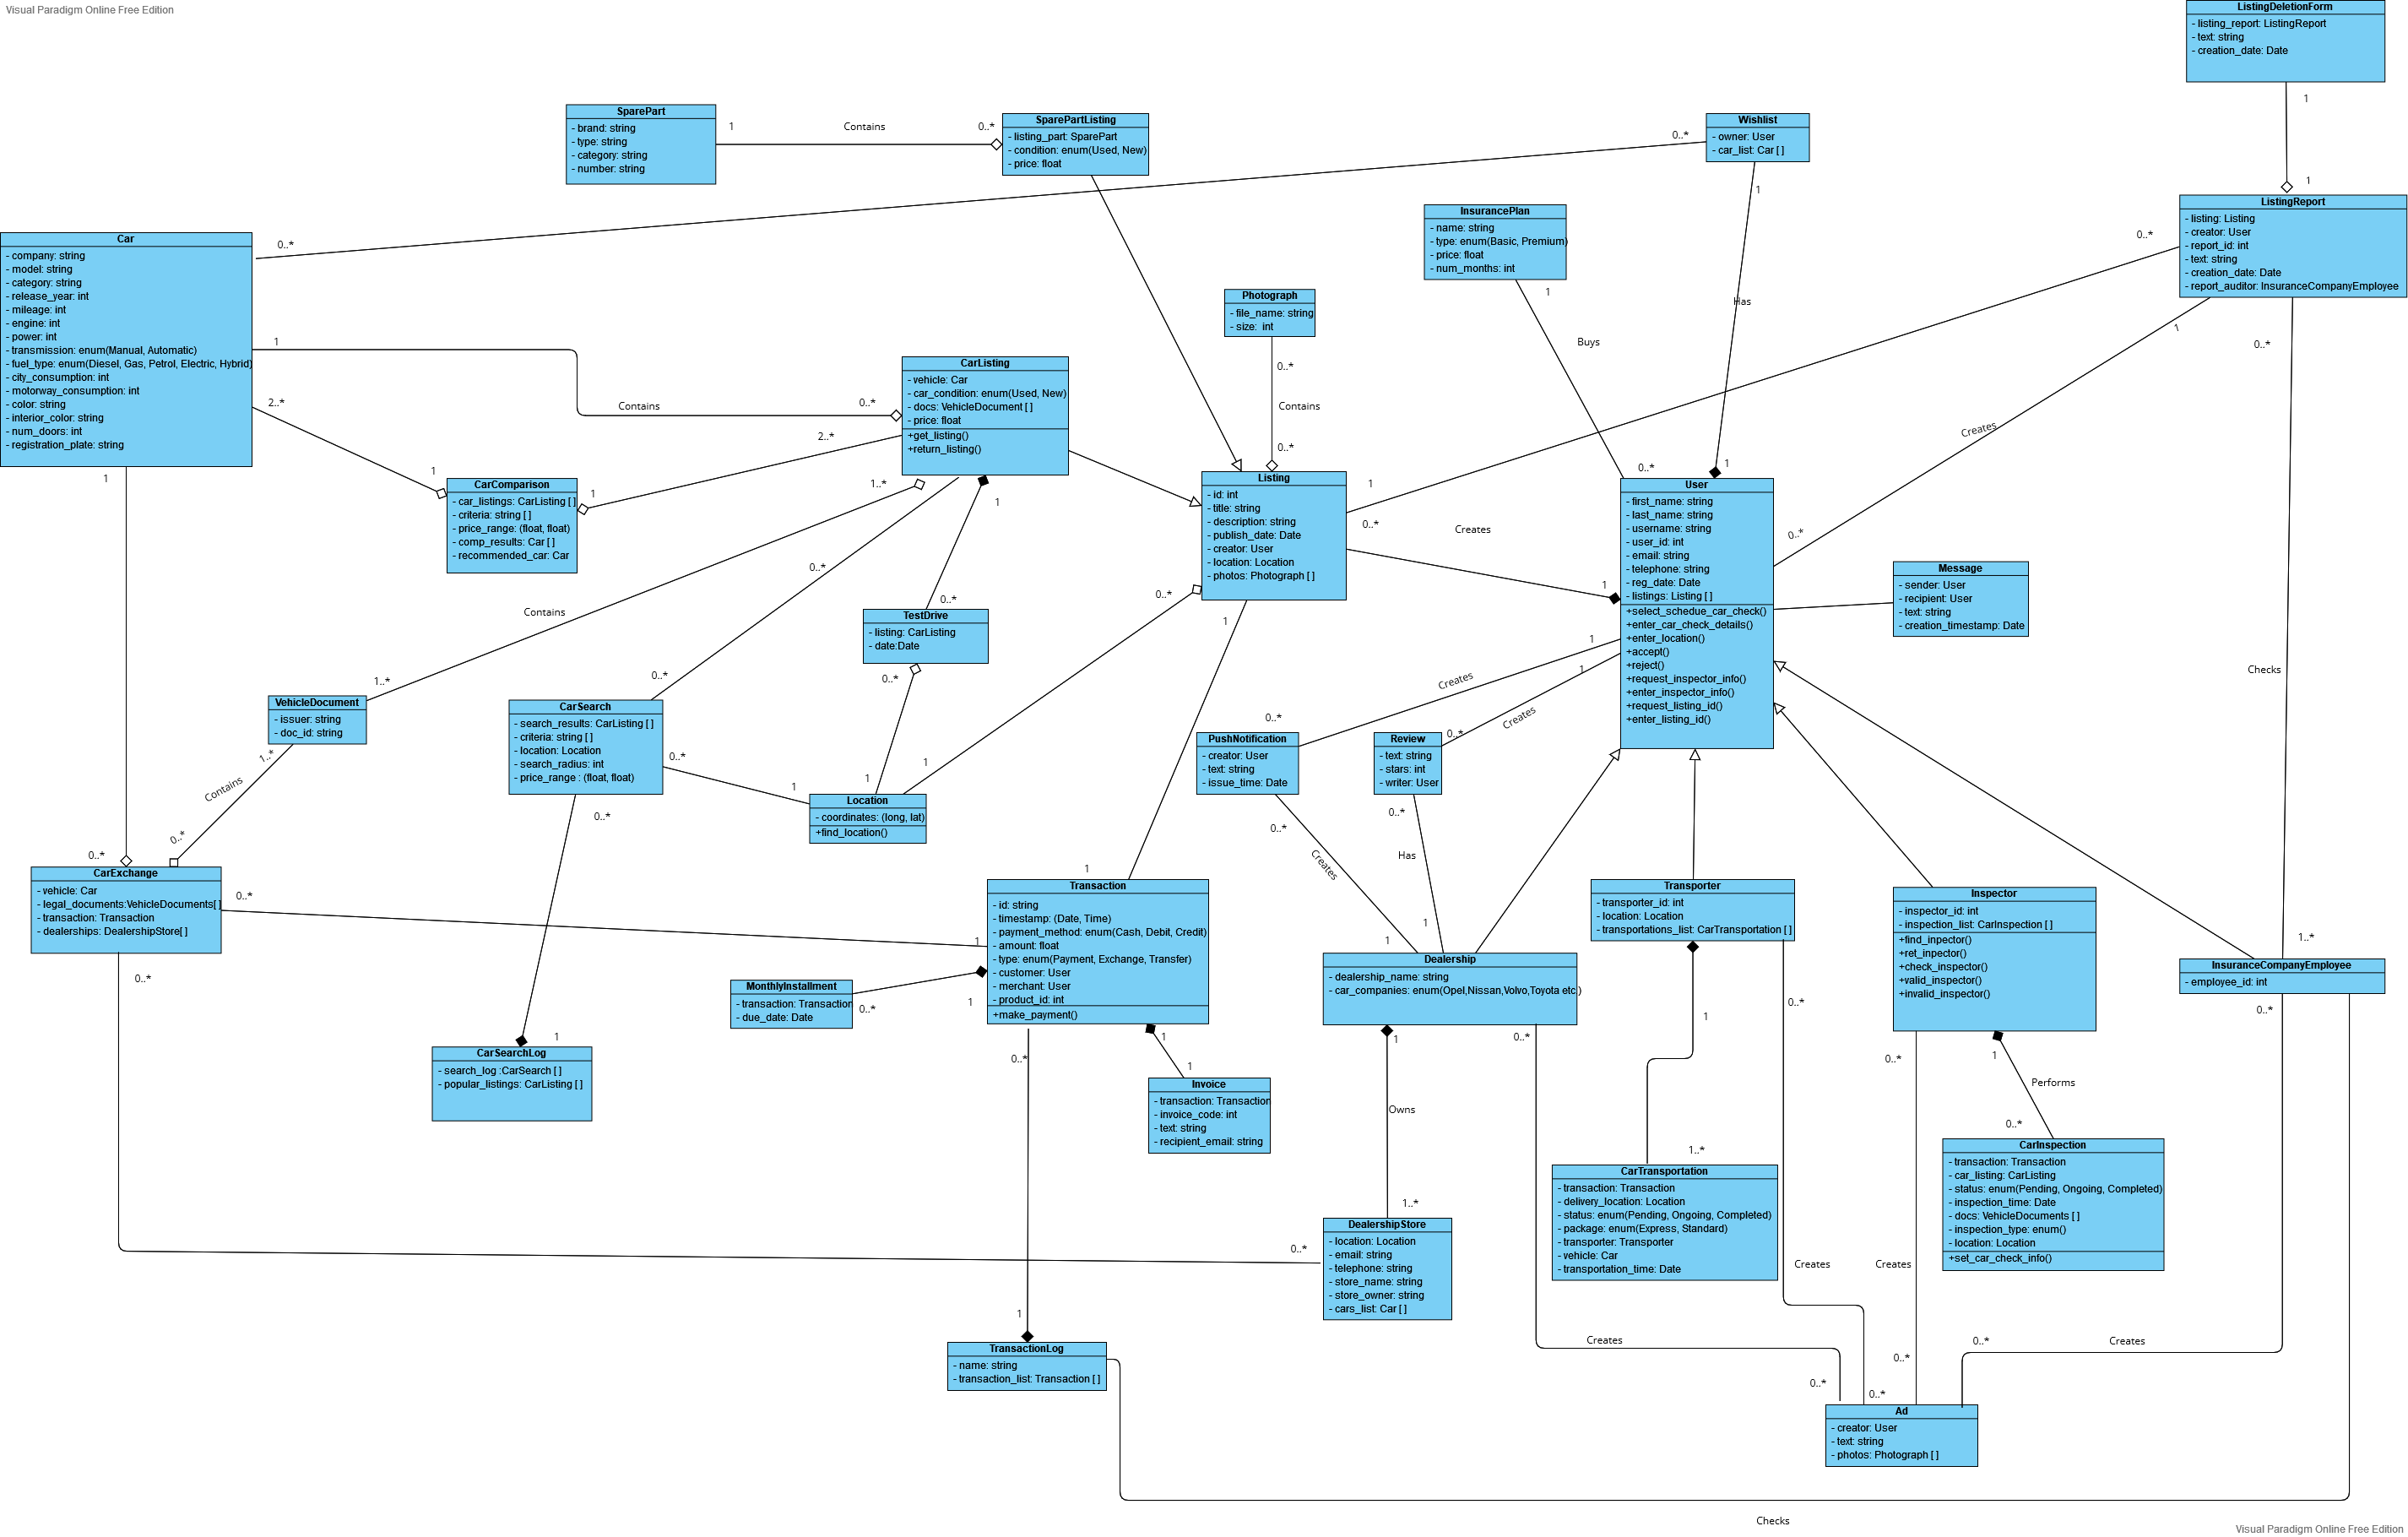
\includegraphics[width=\textwidth+3cm, height=15cm]{img/Domain_model.png}
		\caption{\en Domain Model \gr του \en Project \gr}
	\end{figure}
	
	
	
	\newpage
	
	\center{\textbf{Περιγραφή Κλάσεων}}
	
	\begin{itemize}
		\item \en \textbf{Car} \gr : Οντότητα που αντιστοιχεί σε ένα αυτοκίνητο και περιέχει όλα τα χαρακτηριστικά του (έτος κυκλοφορίας, μοντέλο κλπ)		
		\item \en \textbf{SparePart} \gr : Οντότητα που αντιστοιχεί σε ένα ανταλλακτικό και περιέχει όλα τα χαρακτηριστικά του
		\item \en \textbf{User} \gr : Γενική Οντότητα που αντιστοιχεί στον εγγεγραμμένο χρήστη της πλατφόρμας
		\item \en \textbf{Inspector} \gr : Ειδικότερη περίπτωση εγγεγραμμένου χρήστη, που αντιστοιχεί στους Ελεγκτές που διεξάγουν τους ελέγχους των οχημάτων
		\item \en \textbf{Transporter} \gr : Ειδικότερη περίπτωση εγγεγραμμένου χρήστη, που αφορά τους Μεταφορείς, ευθύνη των οποίων είναι η μεταφορά οχημάτων
		\item \en \textbf{Dealership} \gr : Ειδικότερη περίπτωση εγγεγραμμένου χρήστη, που αντιστοιχεί σε μια Αντιπροσωπεία Οχημάτων
		\item \en \textbf{InsuranceCompanyEmployee} \gr : Ειδικότερη περίπτωση εγγεγραμμένου χρήστη, που αντιστοιχεί σε υπάλληλο της Ασφαλιστικής Εταιρείας που διαχειρίζεται την πλατφόρμα
		\item \en \textbf{Listing} \gr : Οντότητα που αντιστοιχεί σε μια αναρτημένη, στο σύστημα, αγγελία. Μπορεί να είναι είτε αγγελία πώλησης οχήματος (από Ιδιώτη ή από Αντιπροσωπεία), είτε αγγελία πώλησης ανταλλακτικού, είτε αγγελία που έχει αναρτήσει κάποιος Ελεγκτής προκειμένου να πληροφορήσει του χρήστες για τις υπηρεσίες που παρέχει
		\item \en \textbf{CarListing} \gr : Ειδικότερη περίπτωση αναρτημένης αγγελίας, που αφορά αγγελία πώλησης οχήματος
		\item \en \textbf{SparePartListing} \gr : Ειδικότερη περίπτωση αναρτημένης αγγελίας, που αντιστοιχεί σε αγγελία πώλησης ανταλλακτικού
		\item \en \textbf{ListingReport} \gr : Οντότητα που αντιστοιχεί σε Αναφορά αγγελίας και περιέχει χαρακτηριστικά όπως το \en username \gr του δημιουργού της αναφοράς, τον κωδικό της αγγελίας, την αιτία της αναφοράς, κλπ
		\item \en \textbf{Transaction} \gr : Οντότητα που αντιστοιχεί σε μια συναλλαγή που διεξήχθη μέσω της πλατφόρμας και περιέχει όλα τα χαρακτηριστικά της, όπως κωδικός συναλλαγής, ποσό, ημερομηνία κλπ.
		\item \en \textbf{TransactionLog} \gr : Οντότητα που αντιστοιχεί στο μοναδικό και καθολικό Αρχείο Καταγραφής συναλλαγών (\en Log\gr), στο οποίο έχει πρόσβαση μόνο η Ασφαλιστική Εταιρεία
		\item \en \textbf{Message} \gr : Οντότητα που αντιστοιχεί σε μήνυμα που αποστέλλουν μεταξύ τους οι χρήστες της εφαρμογής και περιέχει χαρακτηριστικά όπως το \en username \gr του αποστολέα και του παραλήπτη, την ημερομηνία και ώρα δημιουργίας, κλπ
		\item \en \textbf{Location} \gr : Οντότητα που περιγράφει μια φυσική τοποθεσία και τα χαρακτηριστικά της, όπως το γεωγραφικό της στίγμα
		\item \en \textbf{Advertisment} \gr : Οντότητα που αντιστοιχεί σε μια διαφήμιση που έχει δημιουργηθεί είτε από μια Αντιπροσωπεία, είτε από έναν Μεταφορέα, είτε από έναν Ελεγκτή, είτε από την Ασφαλιστική Εταιρεία
		\item \en \textbf{PushNotification} \gr : Οντότητα που αφορά τα \en Push Notifications \gr που μπορεί να δημιουργήσει μια Αντιπροσωπεία, είτε ειδοποιήσεις που εμφανίζονται στον χρήστη, πχ ως υπενθύμιση για ένα ραντεβού για \en Test Drive \gr
		\item \en \textbf{VehicleDocument} \gr : Οντότητα που αντιστοιχεί σε έγγραφα ενός οχήματος (είτε νομικά είτε πιστοποίησης κατάστασης)  
		\red{\item \en \textbf{CarExchange} \gr : Οντότητα που αφορά μια Ανταλλαγή Οχημάτων που διεξάγεται μεταξύ ενός Ιδιώτη χρήστη και μιας Αντιπροσωπείας. Περιέχει τα στοιχεία του οχήματος, την ανταμοιβή του χρήστη, το \en username \gr του χρήστη και το όνομα της Αντιπροσωπείας}
		\item \en \textbf{CarComparison} \gr : Οντότητα που αντιστοιχεί σε μια σύγκριση μεταξύ οχημάτων, και περιέχει στοιχεία όπως μια λίστα με τα οχήματα που συμμετέχουν στην σύγκριση αλλά και τα κριτήρια με βάση τα οποία γίνεται η σύγκριση
		\item \en \textbf{CarInspection} \gr : Οντότητα που αφορά προγραμματισμένο έλεγχο οχήματος και περιέχει στοιχεία όπως τον κωδικό της αγγελίας του οχήματος και τα χαρακτηριστικά του, τα στοιχεία του Ελεγκτή που θα πραγματοποιήσει τον έλεγχο 
		\item \en \textbf{CarTransporation} \gr : Οντότητα που αντιστοιχεί σε μια προγραμματισμένη μεταφορά οχήματος, και περιέχει στοιχεία όπως την τοποθεσία παράδοσης, τα στοιχεία του παραλήπτη, τα στοιχεία του Μεταφορέα αλλά και τον τύπο της μεταφοράς (Κανονική ή \en Express \gr)
		\item \en \textbf{TestDrive} \gr : Οντότητα που αντιστοιχεί σε ένα προγραμματισμένο ραντεβού για \en Test Drive \gr ενός οχήματος. Περιέχει χαρακτηριστικά όπως τον κωδικό της αγγελίας του οχήματος, την ημερομηνία και ώρα του ραντεβού, το \en username \gr του ενδιαφερόμενου χρήστη
		\item \en \textbf{InsurancePlan} \gr : Οντότητα που αφορά ένα Ασφαλιστικό Πακέτο και περιέχει χαρακτηριστικά όπως τον κωδικό του πακέτου, τα μηνιαία ασφάλιστρα, το \en username \gr του κατόχου του, την ημερομηνία έναρξης και λήξης του συμβολαίου
		\item \en \textbf{MonthlyInstallment} \gr : Οντότητα που αφορά την Μηνιαία Δόση εξόφλησης της αγοράς ενός οχήματος
		\red{\item \en \textbf{Invoice} \gr : Οντότητα που αφορά την Απόδειξη Συναλλαγής} 		
		\item \en \textbf{Review} \gr : Οντότητα που αντιστοιχεί σε κριτική που μπορεί να έχει δεχθεί ένα Ιδιώτης ή μια Αντιπροσωπεία. Περιέχει χαρακτηριστικά όπως το κείμενο της κριτικής, τον αριθμό των αστεριών, το \en username \gr του δημιουργού, την ημερομηνία της δημιουργίας
		\item \en \textbf{Photograph} \gr : Οντότητα που αντιστοιχεί σε μια Φωτογραφία που μπορεί να είναι μέρος μιας αγγελίας πώλησης οχήματος ή ανταλλακτικού
		\item \en \textbf{Wishlist} \gr : Οντότητα που αντιστοιχεί στην \en Wishlist \gr ενός χρήστη
		\item \en \textbf{DealershipStore} \gr : Οντότητα που αντιστοιχεί σε Φυσικό Κατάστημα που υπάγεται σε μια Αντιπροσωπεία Οχημάτων		
	\end{itemize}
	
	
	
	
	
\end{document}
